%%%%%%%%%%%%%%%%% document setup %%%%%%%%%%%%%%%%%

% Don't like 10pt? Try 11pt or 12pt
\documentclass[10pt]{article}

% The automated optical recognition software used to digitize resume
% information works best with fonts that do not have serifs. This
% command uses a sans serif font throughout. Uncomment both lines (or at
% least the second) to restore a Roman font (i.e., a font with serifs).
%\usepackage{times}
%\renewcommand{\familydefault}{\sfdefault}

% This is a helpful package that puts math inside length specifications
\usepackage{calc}
\usepackage{comment}
\usepackage{graphicx}
\graphicspath{ {.} }

% Simpler bibsection for CV sections
% (thanks to natbib for inspiration)
\makeatletter
\newlength{\bibhang}
\setlength{\bibhang}{1em} %1em}
\newlength{\bibsep}
{\@listi \global\bibsep\itemsep \global\advance\bibsep by\parsep}
\newenvironment{bibsection}%
{\begin{enumerate}{}{%
			%        {\begin{list}{}{%
			\setlength{\leftmargin}{\bibhang}%
			\setlength{\itemindent}{-\leftmargin}%
			\setlength{\itemsep}{\bibsep}%
			\setlength{\parsep}{\z@}%
			\setlength{\partopsep}{0pt}%
			\setlength{\topsep}{0pt}}}
	{\end{enumerate}\vspace{-.6\baselineskip}}
%        {\end{list}\vspace{-.6\baselineskip}}
\makeatother

% Layout: Puts the section titles on left side of page
\reversemarginpar

%
%         PAPER SIZE, PAGE NUMBER, AND DOCUMENT LAYOUT NOTES:
%
% The next \usepackage line changes the layout for CV style section
% headings as marginal notes. It also sets up the paper size as either
% letter or A4. By default, letter was used. If A4 paper is desired,
% comment out the letterpaper lines and uncomment the a4paper lines.
%
% As you can see, the margin widths and section title widths can be
% easily adjusted.
%
% ALSO: Notice that the includefoot option can be commented OUT in order
% to put the PAGE NUMBER *IN* the bottom margin. This will make the
% effective text area larger.
%
% IF YOU WISH TO REMOVE THE ``of LASTPAGE'' next to each page number,
% see the note about the +LP and -LP lines below. Comment out the +LP
% and uncomment the -LP.
%
% IF YOU WISH TO REMOVE PAGE NUMBERS, be sure that the includefoot line
% is uncommented and ALSO uncomment the \pagestyle{empty} a few lines
% below.
%

%% Use these lines for letter-sized paper
\usepackage[paper=letterpaper,
%includefoot, % Uncomment to put page number above margin
marginparwidth=1.2in,     % Length of section titles
marginparsep=.05in,       % Space between titles and text
margin=1in,               % 1 inch margins
includemp]{geometry}

%% Use these lines for A4-sized paper
%\usepackage[paper=a4paper,
%            %includefoot, % Uncomment to put page number above margin
%            marginparwidth=30.5mm,    % Length of section titles
%            marginparsep=1.5mm,       % Space between titles and text
%            margin=25mm,              % 25mm margins
%            includemp]{geometry}

%% More layout: Get rid of indenting throughout entire document
\setlength{\parindent}{0in}

\usepackage[shortlabels]{enumitem}

%% Reference the last page in the page number
%
% NOTE: comment the +LP line and uncomment the -LP line to have page
%       numbers without the ``of ##'' last page reference)
%
% NOTE: uncomment the \pagestyle{empty} line to get rid of all page
%       numbers (make sure includefoot is commented out above)
%
\usepackage{fancyhdr,lastpage}
\pagestyle{fancy}
%\pagestyle{empty}      % Uncomment this to get rid of page numbers
\fancyhf{}\renewcommand{\headrulewidth}{0pt}
\fancyfootoffset{\marginparsep+\marginparwidth}
\newlength{\footpageshift}
\setlength{\footpageshift}
{0.5\textwidth+0.5\marginparsep+0.5\marginparwidth-2in}
\lfoot{\hspace{\footpageshift}%
	\parbox{4in}{\, \hfill %
		\arabic{page} of \protect\pageref*{LastPage} % +LP
		%                    \arabic{page}                               % -LP
		\hfill \,}}

% Finally, give us PDF bookmarks
\usepackage{color,hyperref}
\definecolor{darkblue}{rgb}{0.0,0.0,0.3}
\hypersetup{colorlinks,breaklinks,
	linkcolor=darkblue,urlcolor=darkblue,
	anchorcolor=darkblue,citecolor=darkblue}

%%%%%%%%%%%%%%%%%%%%%%%% End Document Setup %%%%%%%%%%%%%%%%%%%%%%%%%%%%


%%%%%%%%%%%%%%%%%%%%%%%%%%% Helper Commands %%%%%%%%%%%%%%%%%%%%%%%%%%%%

% The title (name) with a horizontal rule under it
% (optional argument typesets an object right-justified across from name
%  as well)
%
% Usage: \makeheading{name}
%        OR
%        \makeheading[right_object]{name}
%
% Place at top of document. It should be the first thing.
% If ``right_object'' is provided in the square-braced optional
% argument, it will be right justified on the same line as ``name'' at
% the top of the CV. For example:
%
%       \makeheading[\emph{Curriculum vitae}]{Your Name}
%
% will put an emphasized ``Curriculum vitae'' at the top of the document
% as a title. Likewise, a picture could be included:
%
%   \makeheading[\includegraphics[height=1.5in]{my_picutre}]{Your Name}
%
% the picture will be flush right across from the name.
\newcommand{\makeheading}[2][]%
{\hspace*{-\marginparsep minus \marginparwidth}%
	\begin{minipage}[t]{\textwidth+\marginparwidth+\marginparsep}%
		{\large \bfseries #2 \hfill #1}\\[-0.15\baselineskip]%
		\rule{\columnwidth}{1pt}%
	\end{minipage}}
	
	% The section headings
	%
	% Usage: \section{section name}
	\renewcommand{\section}[1]{\pagebreak[3]%
		\hyphenpenalty=10000%
		\vspace{1.3\baselineskip}%
		\phantomsection\addcontentsline{toc}{section}{#1}%
		\noindent\llap{\scshape\smash{\parbox[t]{\marginparwidth}{\raggedright #1}}}%
		\vspace{-\baselineskip}\par}
	
	% An itemize-style list with lots of space between items
	\newenvironment{outerlist}[1][\enskip\textbullet]%
	{\begin{itemize}[#1,leftmargin=*]}{\end{itemize}%
		\vspace{-.6\baselineskip}}
	
	% An environment IDENTICAL to outerlist that has better pre-list spacing
	% when used as the first thing in a \section
	\newenvironment{lonelist}[1][\enskip\textbullet]%
	{\begin{list}{#1}{%
				\setlength{\partopsep}{0pt}%
				\setlength{\topsep}{0pt}}}
		{\end{list}\vspace{-.6\baselineskip}}
	
	% An itemize-style list with little space between items
	\newenvironment{innerlist}[1][\enskip\textbullet]%
	{\begin{itemize}[#1,leftmargin=*,parsep=0pt,itemsep=0pt,topsep=0pt,partopsep=0pt]}
		{\end{itemize}}
	
	% An environment IDENTICAL to innerlist that has better pre-list spacing
	% when used as the first thing in a \section
	\newenvironment{loneinnerlist}[1][\enskip\textbullet]%
	{\begin{itemize}[#1,leftmargin=*,parsep=0pt,itemsep=0pt,topsep=0pt,partopsep=0pt]}
		{\end{itemize}\vspace{-.6\baselineskip}}
	
	% To add some paragraph space between lines.
	% This also tells LaTeX to preferably break a page on one of these gaps
	% if there is a needed pagebreak nearby.
	\newcommand{\blankline}{\quad\pagebreak[3]}
	\newcommand{\halfblankline}{\quad\vspace{-0.5\baselineskip}\pagebreak[3]}
	
	% Uses hyperref to link DOI
	\newcommand\doilink[1]{\href{http://dx.doi.org/#1}{#1}}
	\newcommand\doi[1]{doi:\doilink{#1}}
	
	% For \url{SOME_URL}, links SOME_URL to the url SOME_URL
	\providecommand*\url[1]{\href{#1}{#1}}
	% Same as above, but pretty-prints SOME_URL in teletype fixed-width font
	\renewcommand*\url[1]{\href{#1}{\texttt{#1}}}
	
	% For \email{ADDRESS}, links ADDRESS to the url mailto:ADDRESS
	\providecommand*\email[1]{\href{mailto:#1}{#1}}
	% Same as above, but pretty-prints ADDRESS in teletype fixed-width font
	%\renewcommand*\email[1]{\href{mailto:#1}{\texttt{#1}}}
	
	%\providecommand\BibTeX{{\rm B\kern-.05em{\sc i\kern-.025em b}\kern-.08em
	%    T\kern-.1667em\lower.7ex\hbox{E}\kern-.125emX}}
	%\providecommand\BibTeX{{\rm B\kern-.05em{\sc i\kern-.025em b}\kern-.08em
	%    \TeX}}
	\providecommand\BibTeX{{B\kern-.05em{\sc i\kern-.025em b}\kern-.08em
			\TeX}}
	\providecommand\Matlab{\textsc{Matlab}}
%%%%%%%%%%%%%%% end docuemnt setup %%%%%%%%%%%%%%%






%%%%%%%%%%%%%%% begin my cv document %%%%%%%%%%%%%%%

\begin{document}
\makeheading[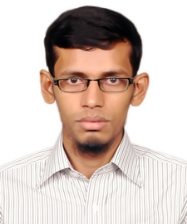
\includegraphics{mahedi}]{Md. Mahedi Hasan}

\section{Contact Information}
\newlength{\rcollength}\setlength{\rcollength}{1.4in}%

\begin{tabular}[t]{@{}p{\textwidth-\rcollength}p{\rcollength}}
	House No: 160/1, Road No: 2, Shahid Nagar,   & +880-1535-822954 \\
	Lalbagh, Dhaka-1211, Bangladesh     & \email{mahedi0803@gmail.com}\\
	Find & \href{http://www.twitter.com/}{Twitter} \href{http://www.github.com/Mahedi-61/}{Github}\\
\end{tabular}


\section{Research Interest}
Computer vision, Image Processing and Pattern Recognition, Machine Learning


\section{Education}
\begin{outerlist}
	\item[] M.Sc. in Information and Communication Technology
		\begin{innerlist}
			\item Bangladesh University of Engineering and Technology (October 2014 - present)
			\item Thesis topic: \emph{Recognizing and tracking people by their gait signature across multiple non-intersecting surveillance cameras.}
			\item Advisor: \href{https://hossenmustafa.buet.ac.bd/} {Dr. Hossen Asiful Mustafa}
			\item CGPA: 3.58 (out of 4)
		\end{innerlist}
	
	\item[] B.Sc. in Electrical and Electronic Engineering
		\begin{innerlist}
			\item Khulna University of Engineering and Technology (September 2013)
			\item Advisor: \href{http://www.kuet.ac.bd/eee/ahmad/} {Prof. Dr. Mohiuddin Ahmad}
			\item CGPA: 3.48 (out of 4)
		\end{innerlist}
		
	\item[] Higher Secondary School Certificate
	\begin{innerlist}
		\item Dhaka Board (July 2008)
		\item Engineering University Higher Secondary School
		\item CGPA: 5.00 (out of 5)
	\end{innerlist}
	
	\item[] Secondary School Certificate
		\begin{innerlist}
			\item Dhaka Board (May 2006)
			\item West End High School
			\item CGPA: 5.00 (out of 5)
		\end{innerlist}
\end{outerlist}

\section{Professional Experience}
\textbf{Adjunct Lecturer} \hfill{May 2016 - present}
	\begin{innerlist}
		\item[]{Manarat International University}
		\item[]{Department of Computer Science and Engineering}
	\end{innerlist}
\flushleft
\textbf{Associate Editor} \hfill{March 2015 - present}
	\begin{innerlist}
		\item[]{Byapon science magazine}
		\item[]{Office: 48/1, Motijheel C/A, Dhaka-1200, Bangladesh}
		\item[]\href{http://www.byapon.com}{Web: www.byapon.com}
	\end{innerlist}



\section{Refereed Journal Publications}
\begin{bibsection}
	\vspace{-.1275in}
	\item {\bf Hasan, M.}, Asiful, H., "Two stream network for gait recognition" \emph{IEEE}, 52(8):25--31, 2018.
	
	\item {\bf Hasan, M.}, Asiful, H., "Bidirectional GRU architecture for human gait recognition" \emph{ICCV}, 201(2):285--292, 2019.
\end{bibsection}

\section{Submitted Journal Publications}
\begin{bibsection}
	\vspace{-.1275in}
	\item {\bf Hasan, M.}, Asiful, H., "Recognizing and tracking people by their gait signatures across multiple non-intersecting surveillance cameras." \emph{IEEE}, 52(8):25--31, 2018.t...
\end{bibsection}

\section{Peer-Reviewed Conference Paper}
\vspace{-.1in}
\begin{bibsection}
	\item {\bf Hasan, M.}, Asiful, H. "preparing journal paper or published conference paper"
\end{bibsection}



\section{Projects}
\begin{outerlist}
	\item  Development of automated essay scoring
	\begin{innerlist}
		\item[] Supervisor: Dr. Hosssen Asiful Mustafa
		\item[] Report \& Code: \href{https://github.com/Mahedi-61/Essay-Scoring/} {https://github.com/Mahedi-61/Essay-Scoring}
	\end{innerlist}

	\item  Development of automated essay scoring
	\begin{innerlist}
		\item[] Supervisor: Dr. Hosssen Asiful Mustafa
		\item[] Report \& Code: \href{https://github.com/Mahedi-61/Essay-Scoring/} {https://github.com/Mahedi-61/Distributed-Password-Cracker}
	\end{innerlist}
	
	\item File Encryption and Decryption with DES
	\begin{innerlist}
		\item[] Supervisor: Dr. Hosssen Asiful Mustafa
		\item[] Report \& Code: \href{https://github.com/Mahedi-61/File-Encryption-Decryption-with-DES} {https://github.com/Mahedi-61/File-Encryption-Decryption-with-DES}
	\end{innerlist}
\end{outerlist}



\section{Achievements}
{\bf B.Sc. Engineering Scholarships}
\begin{innerlist}
	\item[] KUET students merit scholarships through four years for academic
	excellence from the Govt. of the People's Republic of Bangladesh
\end{innerlist}



\section{Extra-Curricular Activities}
\begin{innerlist}
	\item Member at Inter University Tech Fiesta, 2012 Organized by EEE Association, KUET.
	\item Volunteer at IEEE Student Professional Awareness Conference (SPAC), 2010 Organized by IEEE
	Student Branch, KUET.
\end{innerlist}



\section{Technical Skill}
\begin{innerlist}
	\item[] Programming Languages: \hfill {C, C++, Java, Python} \\
	\item[] Hardware: \hfill {Verilog HDL} \\
	\item[] Numerical Analysis: \hfill {MATLAB} \\
	\item[] Application Development: \hfill {Android} \\
	\item[] Database: \hfill {SQL} \\
\end{innerlist}



\section{References}

{\bf Prof. Dr. Md. Liakot Ali}
\begin{innerlist}
	\item[] Professor, \href{http://iict.buet.ac.bd/} {Institute of Information and Communication Technology} (IICT) \\
	\href{http://www.buet.ac.bd/} {Bangladesh University of Engineering and Technology} (BUET) \\
	Dhaka - 1000, Bangladesh \\
    E-mail: liakot@iict.buet.ac.bd  \hfill {Phone: 880-2-55167100/6516}
\end{innerlist}

\halfblankline

{\bf Dr. Hosssen Asiful Mustafa}
\begin{innerlist}
	\item[] Assistant Professor, \href{http://iict.buet.ac.bd/} {Institute of Information and Communication Technology} (IICT \\
	\href{http://www.buet.ac.bd/} {Bangladesh University of Engineering and Technology} (BUET) \\
	Dhaka - 1000, Bangladesh \\
	E-mail: hossen\_mustafa@iict.buet.ac.bd  \hfill {Phone: 880-2-55167100/6208}
\end{innerlist}

\end{document}












